% Extended Abstract

\chapter{Extended Abstract} % Main chapter title

%----------------------------------------------------------------------------------------
\section{Introdução e Enquadramento do Problema}
	A \textit{Critical Techworks} (\textit{CTW}) é uma empresa criada através de uma parceria entre a \textit{Critical Software} e o grupo \textit{BMW}. Desde 2018 que se dedica ao \textbf{desenvolvimento de software} para os vários produtos e serviços digitais da \textit{BMW}. Tendo em conta a quantidade de sistemas ativos e a sua importância, a forma como os incidentes são geridos torna-se um tema essencial para garantir a \textbf{estabilidade dos serviços}.
	
	Um \textbf{incidente} é, na prática, qualquer evento que cause uma \textbf{interrupção} ou  \textbf{degradação} no funcionamento de um serviço. Quando isso acontece, é criado um \textit{ticket} (registo de incidente), com a descrição do problema, a prioridade e outra informação útil para a equipa responsável. Estes incidentes podem resultar de alertas automáticos, baseados em métricas configuradas pelas próprias equipas, ou ser reportados manualmente por utilizadores ou equipas de testes. Em períodos de grande volume de trabalho, ou quando o engenheiro está de prevenção durante a madrugada, é comum surgirem \textbf{dificuldades na interpretação} correta do problema, o que pode levar a erros e aumentar o tempo necessário para encontrar a solução.
	
	O principal desafio identificado é precisamente esta dificuldade em compreender rapidamente o que está a acontecer, sobretudo quando o \textit{ticket} tem pouca informação, é pouco claro ou chega num momento menos favorável. Isto afeta a eficiência das equipas, aumenta o tempo médio de mitigação e pode ter impactos relevantes, tanto a nível financeiro como na experiência de quem utiliza os serviços. Os principais envolvidos neste processo são as equipas de desenvolvimento e operação, os engenheiros de prevenção, os utilizadores internos e externos e a própria organização, que depende da fiabilidade dos seus serviços. O objetivo deste estudo passa por encontrar formas de melhorar a análise dos incidentes e acelerar a sua resolução, reduzindo o impacto que estes problemas podem ter no dia-a-dia da empresa.

\section{Pergunta(s) de Investigação e Objetivos}
	Com base nas dificuldades identificadas pelas equipas \textit{DevOps} e \textit{CorpOps} na análise e resolução de incidentes, surgiu a hipótese de recorrer a ferramentas de Inteligência Artificial, como técnicas de Processamento de Linguagem Natural (\textit{PLN}), para apoiar a compreensão e tratamento destes registos. Desta forma, foi formulada a seguinte questão: “\textbf{Quão eficazes são os Large Language Models na melhoria da interpretação e análise de registos de incidentes de TI?}”.
	
	O objetivo passa por perceber que soluções existem atualmente, de que forma têm sido aplicadas e se há evidências da sua eficácia. Podendo, assim, perceber se existe viabilidade para o desenvolvimento de uma solução que apoie as equipas durante as operações dos seus serviços. Com isso, as equipas poderão conseguir reduzir o Tempo Médio de Resposta (\textit{TMR}) aos incidentes, reduzindo o tempo de indisponibilidade das aplicações, e podendo concentrar maior tempo para o desenvolvimento de outras funcionalidades.

\section{Estado da Arte}
	Optou-se por utilizar um método de pesquisa com base num estudo sistemático de mapeamento (\textit{Systematic Mapping Study} ou \textit{SMS}), a fim de, realizar a revisão de literatura. Primeiramente, foi definida uma pergunta de investigação, para estudar soluções já existentes no mercado, e, de seguida, com base na \textit{RQ} (\textit{Research Question}) definida e com o suporte da metodologia \textit{PICOCS}, foram identificados os elementos necessários para estruturar a pesquisa. Com a questão já enquadrada, prosseguiu-se para definição das palavras chave e dos limites de inclusão e exclusão. Por fim, para obter os artigos, foram utilizadas bases de dados de artigos científicos reconhecidas, tais como, a \textit{ACM Digital Library} e a \textit{IEEE Xplore}.
	
	\subsection{Metodologia PICOC(T)}
		A metodologia \textit{PICOC(T)} é um pequeno guia que ajuda a organizar e a clarificar uma pergunta de investigação. Com esta metodologia podemos dividir o problema em partes simples, como o público-alvo, a solução em análise, o que será comparado e o contexto, tornando mais fácil de perceber exatamente o que se pretende estudar.
		
		\begin{table}[H]
			\centering
			\begin{tabular}{|l|p{3cm}|p{3cm}|p{4cm}|}
				\hline
				\textbf{PICOCT} & \textbf{RQ part} & \textbf{I/E} & \textbf{Sub String} \\
				\hline
				\textbf{P – População} & Registos de incidentes & I — Ferramenta ServiceNow\newline 
				
				E — Estudos sobre gestão de alarmes & "incident management"; "incident analysis"; "incident resolution"; "incident interpretation"; "ticket analysis"; "ticket interpretation"; "ServiceNow" \\
				\hline
				\textbf{I – Intervenção} & Uso de LLMs para análise de incidentes & I — Técnicas conhecidas de LLMs\newline
				
				E — - - - & "Large Language Model"; "LLM"; "Natural Language Processing"; "NLP"; "RAG"; "fine-tuning" \\
				\hline
				\textbf{C – Comparação} & ——— & ——— & ——— \\
				\hline
				\textbf{O – Outcome} & Redução do MTTR, melhoria na priorização e diminuição de erros de analise & I — - - -\newline
				
				E — Estudos não relacionados com incidentes & "incident"; "ticket" \\
				\hline
				\textbf{C – Contexto} & Ambientes DevOps/CorpOps & I — Estudos na área\newline
				
				E — Estudos fora da área & "DevOps"; "CorpOps"; "IT"\\
				\hline
				\textbf{T – Tipo de estudo} & Pesquisa empírica ou com base em estudos & I — - - -\newline
				
				E — Trabalho teórico ou especulativo & Exclude —> "theoretical"; "speculative" \\
				\hline
			\end{tabular}
			\caption[Metodologia PICOCT]{Metodologia PICOCT}
			\label{tab:picocs}
		\end{table}


	\subsection{Palavras Chave Utilizadas}
		\lstset{language=Java}
		\begin{lstlisting}
			("incident management" OR "incident analysis" OR "incident resolution" OR "incident interpretation" OR "ticket analysis" OR "ticket interpretation" OR "ServiceNow")
			AND
			("Large Language Model" OR "LLM" OR "Natural Language Processing" OR "NLP" OR "RAG" OR "fine-tuning")
			AND
			("incident" OR "ticket")
			AND
			("DevOps" OR "CorpOps" OR "IT")
			NOT
			("theoretical" OR "speculative")
		\end{lstlisting}
	
	\subsection{Critérios de Inclusão e Exclusão}
		Para reduzir o “ruído” resultante das bases de dados e melhorar a eficácia da revisão de literatura, foi decidido \textbf{excluir} artigos com mais de 5 anos e \textbf{incluir} apenas os que eram provenientes das conferências mais relacionadas com o tema, como a \textit{International Conference on Software Engineering} (\textit{ICSE}), a \textit{ACM Joint European Software Engineering Conference and Symposium on the Foundations of Software Engineering} (\textit{ESEC/FSE}) e a conferência \textit{Automated Software Engineering} (ASE\textit{}). 
		
	\subsection{PRISMA}
		Para organizar a revisão de literatura, recorreu-se ao método \textit{PRISMA}, que ajuda a tornar o processo de seleção de estudos \textbf{mais claro e transparente}. No total, foram \textbf{identificados 61 artigos} (provenientes do \textit{ACM} e \textit{IEEE Xplore}), dos quais \textbf{1 foi removido por ser duplicado}. Seguiu-se a filtragem por tipo de publicação, \textbf{excluindo 26 artigos} de conferências que não se enquadravam no âmbito pretendido. Depois, a leitura dos resumos levou à \textbf{remoção de mais 29 artigos }por falta de relevância. No final, \textbf{permaneceram 5 artigos} que cumprem os critérios definidos e servem de base à análise realizada.
		
		Para o artigo final serão incluídos mais bases de dados a fim de analisar um número maior de estudos.
		
	\subsection{Principais trabalhos revistos}
		Dos artigos resultantes da metodologia \textit{PRISMA}, foram analisados os principais objetivos e conclusões dos respetivos estudos.
		
		\subsubsection{Artigo 1 - Exploring LLM-Based Agents for Root Cause Analysis}
			Esta investigação destaca um problema comum vivido pelos \textit{OCE}'s (\textit{On Call Engeinners}) aquando de um incidente. As pessoas em operações têm de determinar a causa do incidente para o poder resolver da forma mais eficaz, a este processo chama-se \textit{Root Cause Analysis} (\textit{RCA}). Desta forma, o estudo em questão apura soluções, com o uso de \textit{LLM}'s, para automatizar este processo de análise gerando sugestões aos engenheiros que permitam uma mitigação dos incidentes mais eficiente. Este estudo apoia-se não só no histórico de instruções como também em ferramentas complementares de registos de logs. No final do ensaio, o autor afirma que os comentários deixados nos incidentes não têm grande impacto na performance dos agentes de \textit{LLM}, porém o estudo baseou-se apenas em datasets estáticos o que pode enviesar esta análise. (Roy et al., 2024)
	
		\subsubsection{Artigo 2 - How to mitigate the incident? an effective troubleshooting guide recommendation technique for online service systems}
			Este estudo, expõe os Guias de mitigação de incidentes (ou \textit{TSG} - \textit{Troubleshooting Guides}) como um passo importante na gestão dos incidentes por parte dos \textit{OCE}'s. Tem como \textbf{objetivo investigar o uso e as características dos TSG's} e posteriormente o desenvolvimento de uma ferramenta capaz de identificar os melhores guias de mitigação tendo em conta as descrições dos incidentes. Com esta análise foi possível perceber que ~27\% dos incidentes têm guias correspondentes, o que não se aplica ao nosso dataset, e que ~36\% dos guias ocorriam mais do uma vez por ano, evidenciando a existência de incidentes semelhantes ao longo do ano. Com isto, é possível perceber a importância da análise de incidentes anteriores para a análise e mitigação de incidentes futuros. No final, foi possível concluir que em ~80\% dos incidentes registados, a ferramenta foi capaz de sugerir o \textit{TSG} mais adequado no Top 1. (Jiang et al., 2020)
		
		\subsubsection{Artigo 3 - Identifying linked incidents in large-scale online service systems}
			Neste artigo, foi apresentado um estudo para a criação da ferramenta \textit{LiDAR} (\textit{Linked Incident identification with DAta-driven Representation}), com o \textbf{objetivo de ligar incidentes semelhantes, duplicados ou com a mesma origem}. Os estudos e as experiências realizadas permitiram afirmar que a ferramenta desenvolvida foi efetiva e facilmente aplicada pelos \textit{OCE}'s e que facilitou a gestão de incidentes em sistemas mais complexos. (Chen et al., 2020)
		
		\subsubsection{Artigo 4 - X-Lifecycle Learning for Cloud Incident Management using LLMs}
			Esta análise \textbf{focou-se em quantificar a importância de melhorar os prompts realizados} aos \textit{LLM}'s com dados reais de diferentes etapas do ciclo de vida do software. É algo importante para o estudo a ser realizado aqui mas mais a longo termo. (Goel et al., 2024)
		
		\subsubsection{Artigo 5 - Xpert: Empowering Incident Management with Query Recommendations via Large Language Models}
			Esta pesquisa, apesar de ainda se concentrar no tema de gestão de incidentes, foca um pouco mais da sua investigação na \textbf{recomendação e geração de queries} (\textit{KQL}) para ajudar os \textit{OCE}'s na investigação e mitigação dos incidentes. Novamente, algo que seria um trabalho mais futuro para a proposta inicialmente apresentada neste estudo. (Jiang et al., 2024)
		
	\subsection{Conclusão dos trabalhos revistos}
		 \textbf{Identificar corretamente incidentes} ligados não só ajuda na \textbf{mitigação de incidente}, como também na \textbf{identificação da sua origem} (Chen et al., 2020). Isto é importante para o estudo a realizar, uma vez que uma das premissas é a sugestão dos passos para mitigar os problemas.
		
		Esta investigação vem, assim, juntar um pouco dos artigos apresentados anteriormente de forma a gerar uma solução capaz de analisar incidentes anteriores e sugerir passos para mitigar os incidentes de uma forma eficaz, isto inclui também a análise de registos dos próprios serviços.

\section{Metodologia Proposta}
	Com análise dos artigos anteriores, é possível afirmar que, \textbf{no mercado já existem estudos e ferramentas} usadas em testes capazes resolver o problema mencionado a cima. Porém \textbf{não existe uma ferramenta única} que agregue todas as funcionalidade pretendidas, tais como, a análise do histórico dos registos dos incidentes, a geração de uma descrição em Linguagem Natural para cada incidente e a sugestão de possíveis formas de mitigar os incidentes, assim como, a integração com um serviço externo, como ferramentas de visualização de dados dos serviços.
	
	\begin{figure}[H]
		\centering
		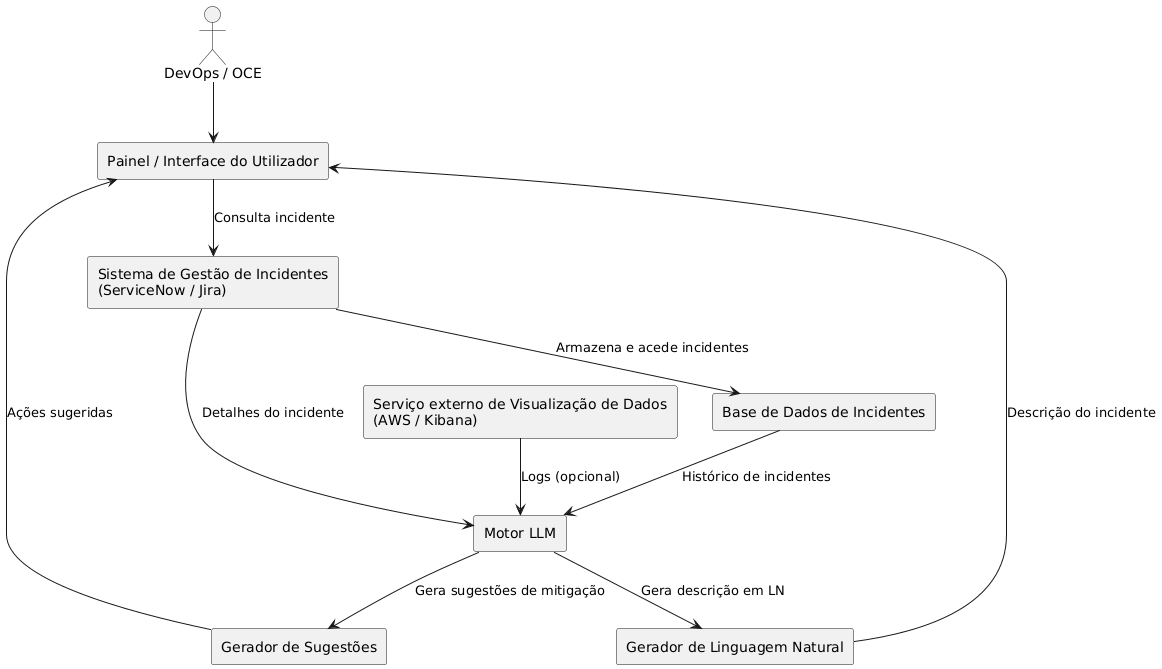
\includegraphics[width=\textwidth,keepaspectratio]{img/diagrama_componentes}
		\caption[Diagrama da Solução Proposta]{Diagrama da Solução Proposta}
		\label{fig:diagramaComponentes}
	\end{figure}


\section{Plano de Trabalho}

	\begin{figure}[H]
		\centering
		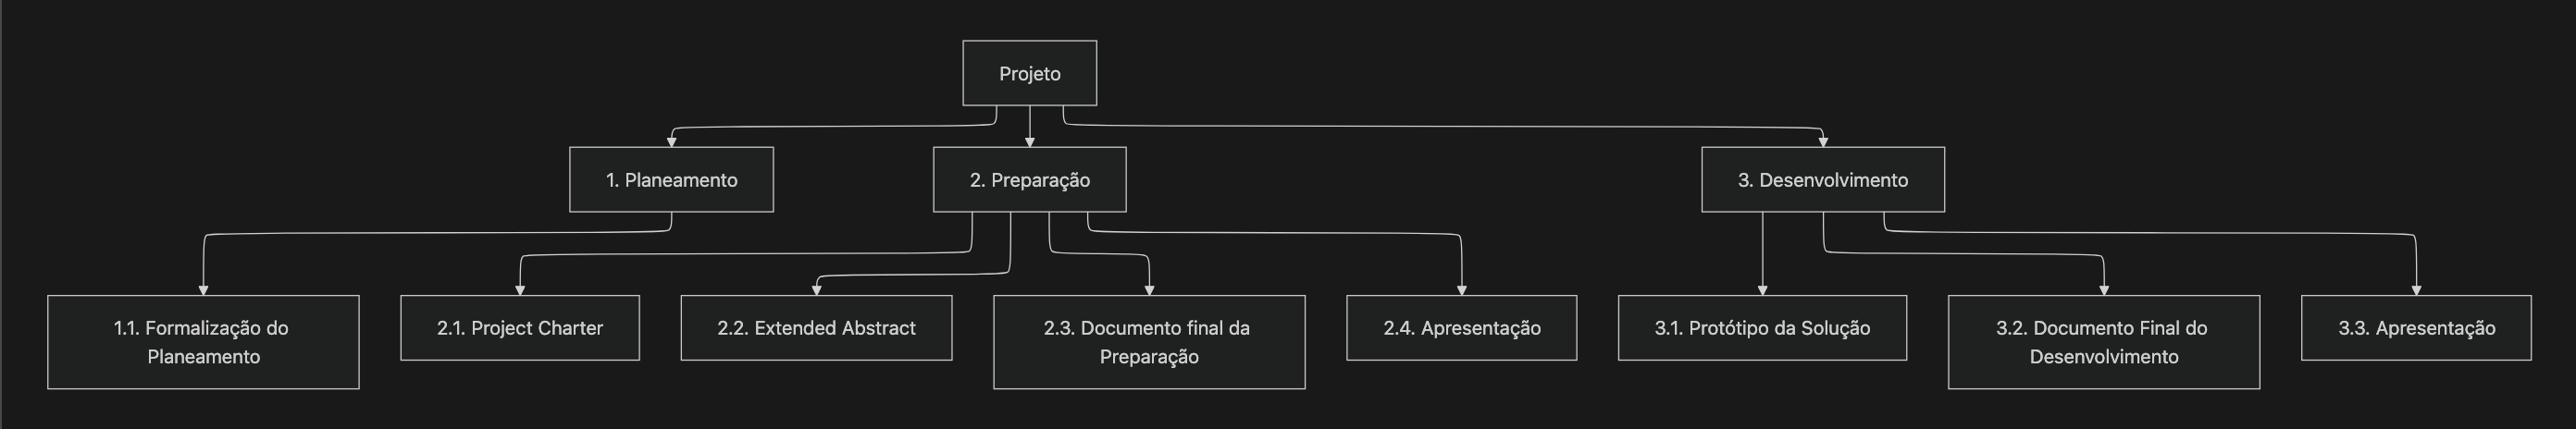
\includegraphics[width=\textwidth,keepaspectratio]{img/wbs}
		\caption[Estrutura Analítica do Projeto]{Estrutura Analítica do Projeto}
		\label{fig:wbs}
	\end{figure}
	\begin{figure}[H]
		\centering
		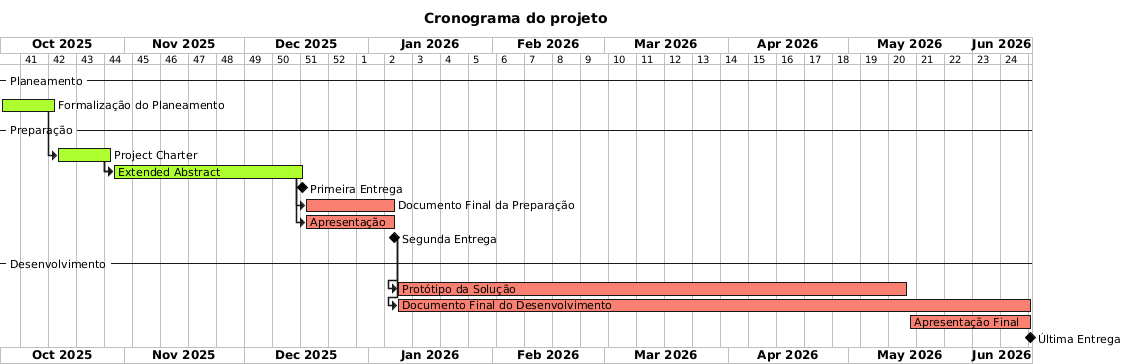
\includegraphics[width=\textwidth,keepaspectratio]{img/cronograma_inicial}
		\caption[Cronograma do Projeto]{Cronograma do Projeto}
		\label{fig:ganttChart}
	\end{figure}

\section{Considerações Éticas e Profissionais}
	Neste projeto, foram seguidos os princípios dos códigos de ética da \textit{ACM} (\textit{Code of Ethics and Professional Conduct}), \textit{NSPE} (\textit{Code of Ethics for Engineers}) e da \textit{ACM/IEEE-CS} (\textit{Software Engineering Code}), de forma a orientar o estudo a atuar com responsabilidade, tanto em relação aos dados como às pessoas afetadas pela solução.
	
	Tendo em conta os dados a serem utilizados poderem \textbf{incluir informações confidenciais}, foi avaliada cuidadosamente a possibilidade de anonimizar os dados e, caso não seja satisfatório para as partes interessadas, será garantido que apenas os resultados agregados sejam apresentados, \textbf{evitando quaisquer riscos de exposição de dados confidenciais}. Não identificámos outros riscos éticos relevantes no projeto.
	
	Para além dos códigos acima mencionados, foi também seguido o Código de Boas Práticas e de Conduta do Instituto Politécnico do Porto.
	
	Quanto às competências necessárias, o autor é também um dos muitos engenheiros que lidam com o tipo de problema que este projeto aborda, estando também a aprofundar os conceitos no mestrado que originou esta investigação. Essa combinação de experiência na área e aprendizagem académica ajuda a assegurar que o trabalho é feito com rigor, ética e atenção às melhores práticas profissionais.


\section{Referências Bibliográficas}

[1]

D. Roy *et al.*, «Exploring LLM-Based Agents for Root Cause Analysis», em *Companion Proceedings of the 32nd ACM International Conference on the Foundations of Software Engineering*, em FSE 2024. New York, NY, USA: Association for Computing Machinery, 2024, pp. 208–219. doi: [10.1145/3663529.3663841](https://doi.org/10.1145/3663529.3663841).

[2]

J. Jiang *et al.*, «How to mitigate the incident? an effective troubleshooting guide recommendation technique for online service systems», em *Proceedings of the 28th ACM Joint Meeting on European Software Engineering Conference and Symposium on the Foundations of Software Engineering*, em ESEC/FSE 2020. New York, NY, USA: Association for Computing Machinery, 2020, pp. 1410–1420. doi: [10.1145/3368089.3417054](https://doi.org/10.1145/3368089.3417054).

[3]

Y. Chen *et al.*, «Identifying linked incidents in large-scale online service systems», em *Proceedings of the 28th ACM Joint Meeting on European Software Engineering Conference and Symposium on the Foundations of Software Engineering*, em ESEC/FSE 2020. New York, NY, USA: Association for Computing Machinery, 2020, pp. 304–314. doi: [10.1145/3368089.3409768](https://doi.org/10.1145/3368089.3409768).

[4]

D. Goel *et al.*, «X-Lifecycle Learning for Cloud Incident Management using LLMs», em *Companion Proceedings of the 32nd ACM International Conference on the Foundations of Software Engineering*, em FSE 2024. New York, NY, USA: Association for Computing Machinery, 2024, pp. 417–428. doi: [10.1145/3663529.3663861](https://doi.org/10.1145/3663529.3663861).

[5]

Y. Jiang *et al.*, «Xpert: Empowering Incident Management with Query Recommendations via Large Language Models», em *Proceedings of the IEEE/ACM 46th International Conference on Software Engineering*, em ICSE ’24. New York, NY, USA: Association for Computing Machinery, 2024. doi: [10.1145/3597503.3639081](https://doi.org/10.1145/3597503.3639081).
